\documentclass[tikz,border=10pt]{standalone}
\usetikzlibrary{calc,angles,quotes}

\begin{document}
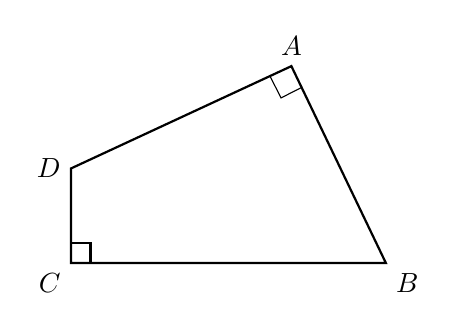
\begin{tikzpicture}[>=stealth, thick]
    % 1. 定义坐标点 (基于图像比例设定)
    % 设定 C 为原点，BC 在水平线上
    \coordinate (C) at (0,0);
    \coordinate (B) at (4,0);
    \coordinate (D) at (0,1.2);
    
    % 计算 A 点：由角 DAB=90度 且位于适当位置推导
    % 这里根据原图视觉比例，设定 A 的坐标
    \coordinate (A) at (2.8,2.5);

    % 2. 绘制四边形边界
    \draw (A) -- (B) -- (C) -- (D) -- cycle;

    % 3. 绘制直角符号
    % 绘制 C 点处的直角
    \draw (0.25,0) -- (0.25,0.25) -- (0,0.25);
    
    % 绘制 A 点处的直角 (需要旋转以适应边 AB 和 AD 的斜率)
    \begin{scope}[shift={(A)}, rotate around={-63:(A)}]
        \draw[thin] (0,-0.3) -- (0.3,-0.3) -- (0.3,0);
    \end{scope}

    % 4. 标注顶点文字
    % anchor 调整文字相对于坐标点的方位，确保不与线段重叠
    \node[above] at (A) {$A$};
    \node[below right] at (B) {$B$};
    \node[below left] at (C) {$C$};
    \node[left] at (D) {$D$};

\end{tikzpicture}
\end{document}